\chapter{SYSTEM DESIGN}\label{ch:design}

\section{System Architecture}\label{sec:architecture}

\begin{figure}[h]
  \centering
  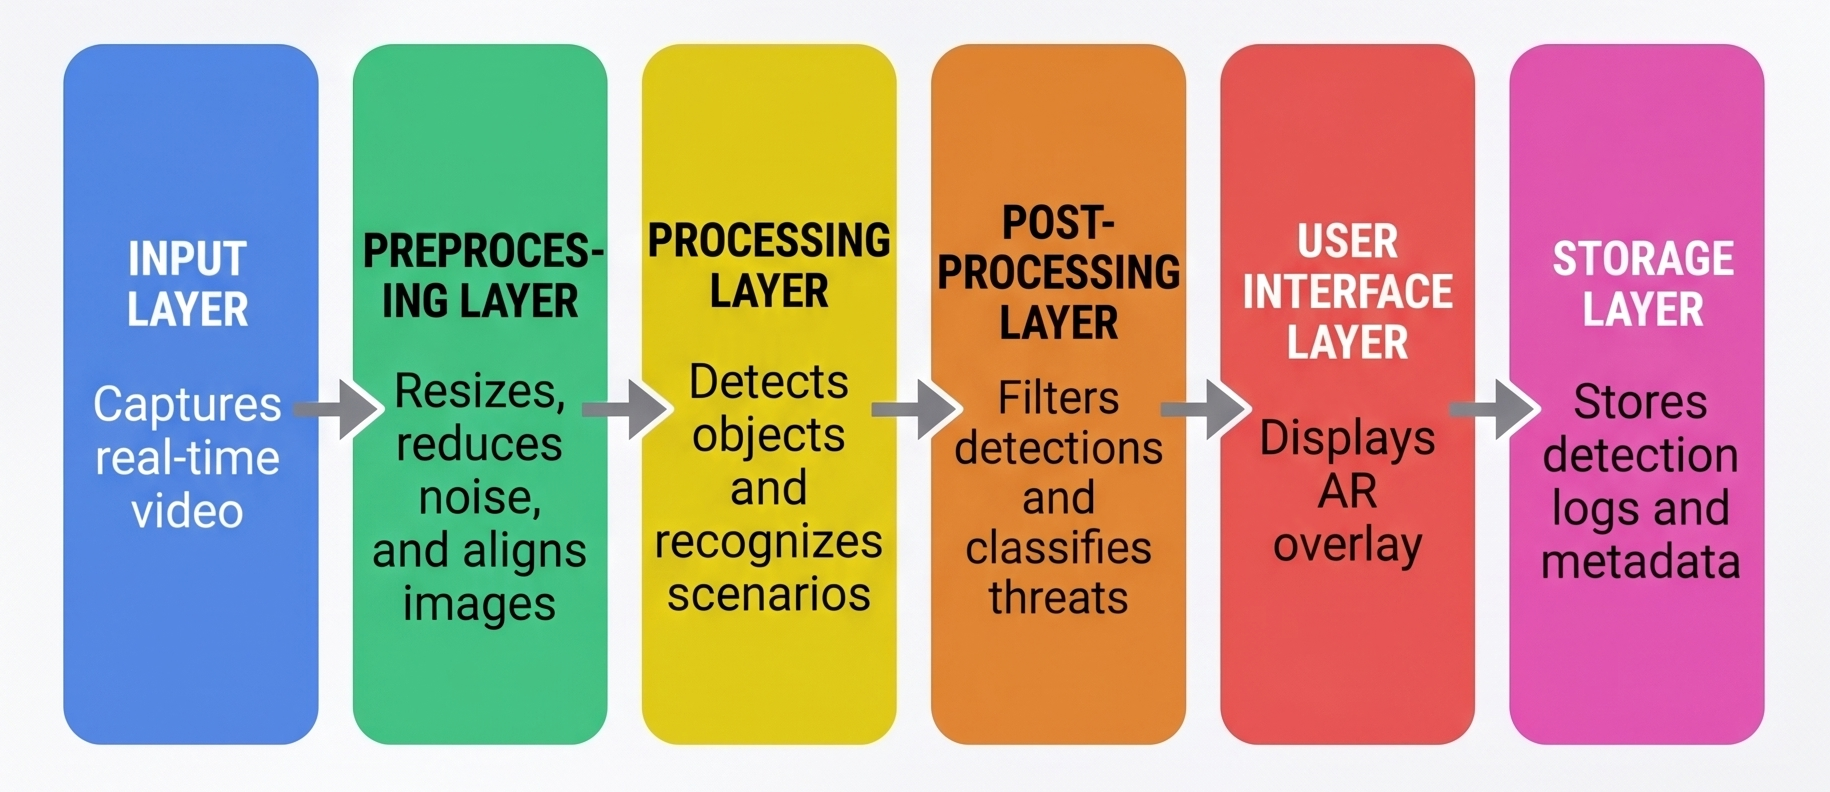
\includegraphics[width=0.9\textwidth]{images/architecture.png}
  \caption{System Architecture}\label{fig:architecture}
\end{figure}

The system architecture for the project is structured into six distinct layers that facilitate a
smooth data flow from capture to storage. It begins with the Input Layer, which is responsible for
capturing real-time video footage. This raw data is then passed to the Preprocessing Layer, where
images are resized, aligned, and noise is reduced to ensure clarity for analysis. The Processing
Layer serves as the core intelligence hub, detecting objects and recognizing specific scenarios,
followed by the Post-Processing Layer, which filters these detections and classifies potential
threats. Finally, the User Interface Layer provides an interactive experience by displaying an AR
overlay of the results, while the Storage Layer logs all detection data and metadata for future
reference.

\label{end:architecture}
\section{System Workflow}\label{sec:workflow}
\begin{figure}[h]
  \centering
  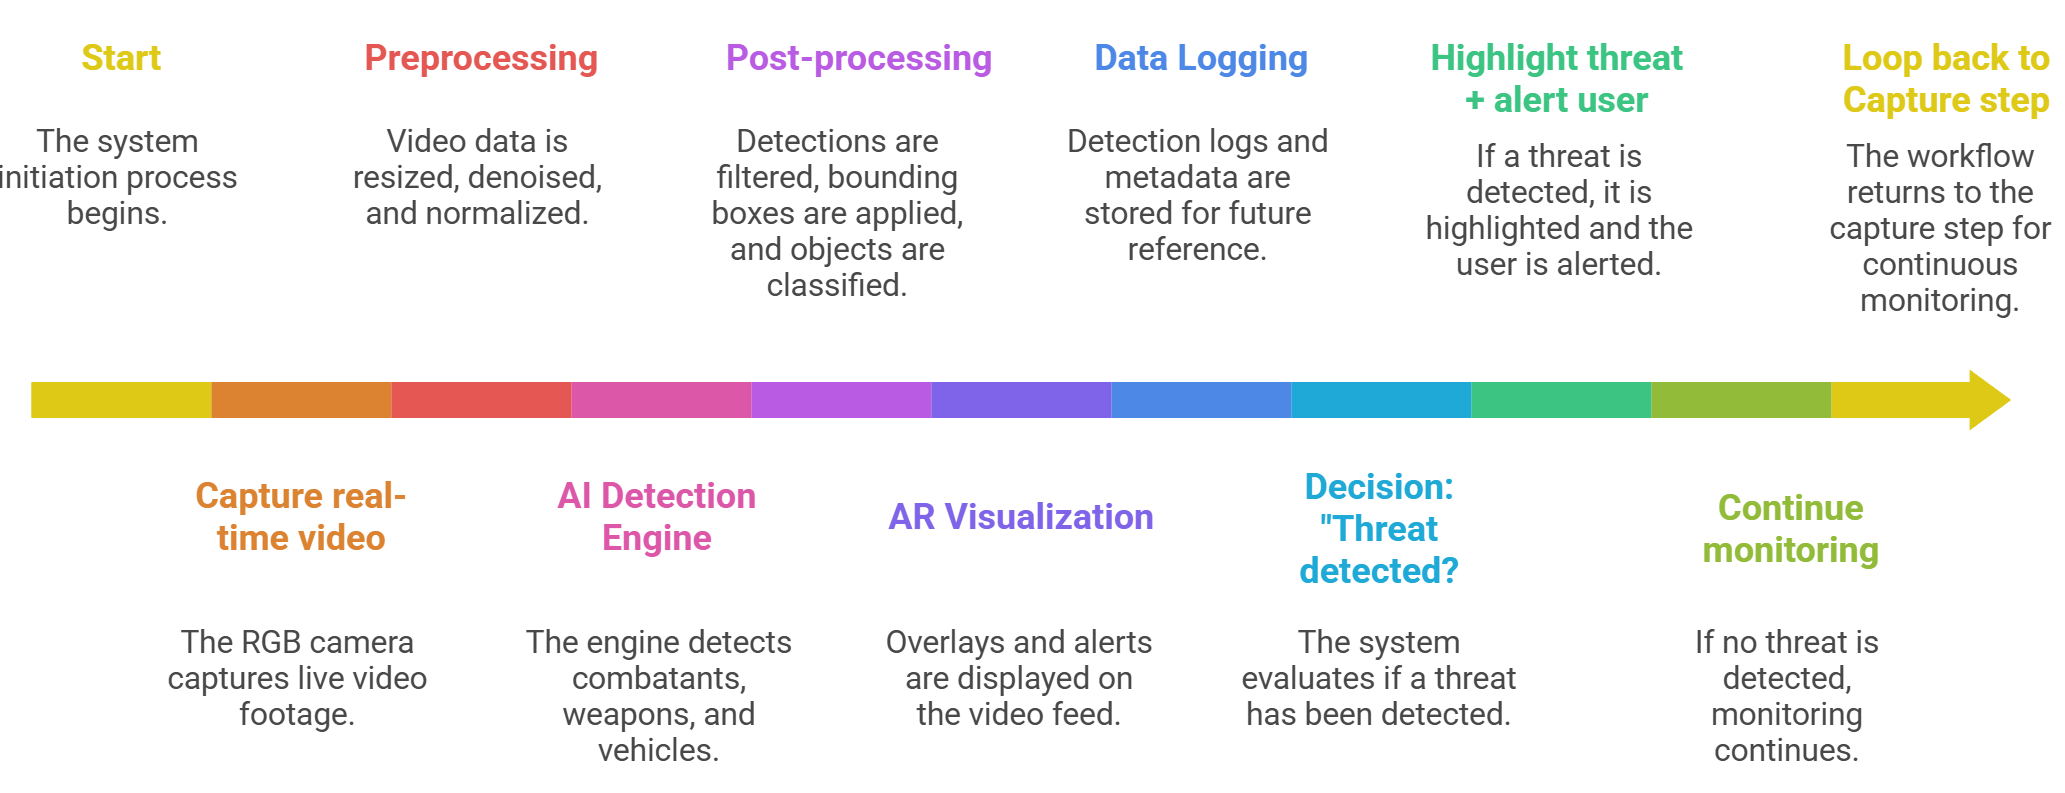
\includegraphics[width=0.9\textwidth]{images/workflow.png}
  \caption{System Workflow}\label{fig:workflow}
\end{figure}

The workflow follows a continuous loop designed for real-time monitoring and rapid response. Upon
initiation, the system captures live RGB video and immediately subjects it to preprocessing steps
like denoising and normalization. The AI Detection Engine then analyzes the feed to identify
combatants, weapons, or vehicles. This leads to a critical decision point: if a threat is detected,
the system applies bounding boxes, highlights the danger via AR visualization, alerts the user, and
logs the data. If no threat is found, the system simply continues its monitoring cycle, returning to
the capture step to ensure persistent surveillance.
\label{end:workflow}\label{end:design}
